% Codebook as k-means / Voronoi partition — TikZ source. Compiles to a tight
% standalone PDF (pdflatex figures/voronoi-kmeans.tex), which
% `book-scaffold build-figures` converts to public/figures/voronoi-kmeans.svg.
%
% Three code vectors (large dots) partition latent space into Voronoi cells;
% encoder outputs (small dots) are assigned to the nearest code; each code is
% the centroid of its assigned points (Lloyd's update).
\documentclass[tikz,border=3pt]{standalone}
\usepackage{amsmath}
\usepackage{amssymb}
\usepackage{tikz}
\usetikzlibrary{positioning,arrows.meta,calc}
\begin{document}
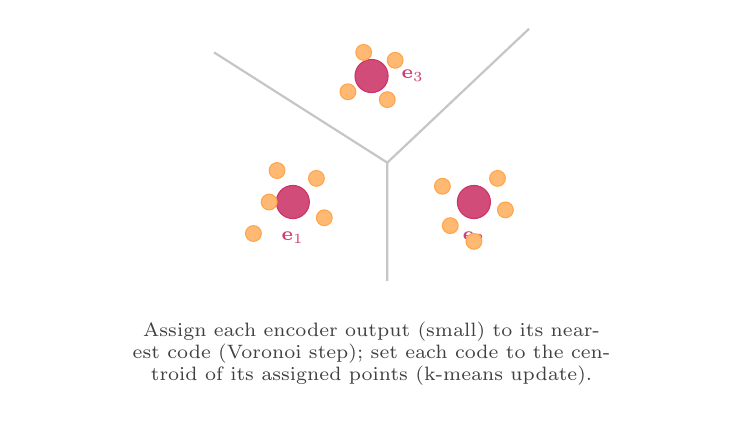
\begin{tikzpicture}[
    font=\small, scale=1.0,
    code/.style={circle, fill=purple!70, draw=purple!80, inner sep=0pt,
                 minimum size=4.2mm},
    pt/.style={circle, fill=orange!55, draw=orange!70, inner sep=0pt,
               minimum size=2.0mm},
    cell/.style={gray!45, thick},
  ]
  % approximate Voronoi boundaries (three cells) as two bisecting segments
  \draw[cell] (2.4,0) -- (2.4,1.5) -- (4.2,3.2);
  \draw[cell] (2.4,1.5) -- (0.2,2.9);

  % code vectors (centroids)
  \node[code] (e1) at (1.2,1.0) {};
  \node[code] (e2) at (3.5,1.0) {};
  \node[code] (e3) at (2.2,2.6) {};
  \node[font=\scriptsize, text=purple!75, below=0.4mm of e1] {$\mathbf e_1$};
  \node[font=\scriptsize, text=purple!75, below=0.4mm of e2] {$\mathbf e_2$};
  \node[font=\scriptsize, text=purple!75, right=0.4mm of e3] {$\mathbf e_3$};

  % encoder outputs assigned to each cell (small dots near each centroid)
  \foreach \p in {(0.7,0.6),(1.0,1.4),(1.6,0.8),(0.9,1.0),(1.5,1.3)}
    \node[pt] at \p {};
  \foreach \p in {(3.2,0.7),(3.8,1.3),(3.5,0.5),(3.9,0.9),(3.1,1.2)}
    \node[pt] at \p {};
  \foreach \p in {(1.9,2.4),(2.5,2.8),(2.1,2.9),(2.4,2.3)}
    \node[pt] at \p {};

  \node[below, align=center, text width=8.5cm, font=\scriptsize, text=black!75]
    at (2.2,-0.4)
    {Assign each encoder output (small) to its nearest code (Voronoi step); set each
     code to the centroid of its assigned points (k-means update).};
\end{tikzpicture}
\end{document}
